\pdfoutput=1
\documentclass[amssymb,aps,twocolumn]{article}
%\documentclass[reprint,pre,aps]{revtex4-1}
\usepackage{amsmath}    % need for subequations
\usepackage{verbatim}   % useful for program listings
%\usepackage{hyperref}   % use for hypertext links, including those to external \bibliographystyle{ieeetr}
%\usepackage{cleveref}

\usepackage{fullpage}
%\usepackage[utf8]{inputenc}
%\usepackage{fullpage}
\usepackage{graphicx,color}
\bibliographystyle{ieeetr}
%\usepackage{xfrac}
\usepackage{amssymb}
%\usepackage{floatrow}
%\usepackage{caption}
\usepackage{subcaption}

% Nature citation format
%\usepackage[space]{cite}
%\usepackage{citesupernumber}
%\usepackage{numberlabel}  % nature.sty is deprecated
%\bibliographystyle{ieee}

% Customizing captions and float behavior
%\usepackage[format=plain,labelformat=empty,font=small]{caption}
%\usepackage{placeins}

% For creating nice looking tables
%\usepackage{booktabs}
%\usepackage{multirow}
\usepackage{authblk}
\renewcommand{\thesection}{}
\renewcommand{\thesubsection}{\alph{subsection}}
\usepackage{sectsty}
\sectionfont{\bfseries\large\center}
\subsectionfont{\bfseries\normalsize\center}
% Choose your font: uncomment one of the below font packages or add your own
%\usepackage{pslatex} % for TNR
%\usepackage{palatino} % for Palatino
%\usepackage{fontspec} % forces XeLaTeX engine, use \setmainfont (etc) below
% \setmainfont[Mapping=tex-text,Ligatures=TeX]{Adobe Caslon Pro} % choose any system font
% \setmainfont[Mapping=tex-text]{Hoefler Text} % ...such as Hoefler Text


\begin{document}
%!TEX root = main.tex
Title
% Title ideas:
%


%%!TEX root = main.tex

\section*{Abstract}

\lipsum[1]

%!TEX root = CS_ORNs.tex

{\color{blue} Intro forthcoming}

\section{Results}

\subsection{A model of odor encoding that preserves ORN tuning, diversity, and adaptive scaling}

{\color{blue}Add introduction to the motivation for the model here. Discuss adaptation found in SG-S and Vijay's work.}


The theoretical framework of odor discrimination consists of two stages: a biophysical model of odor binding and subsequent ORN firing -- encoding -- and a computational paradigm for then inferring odor identity and intensity from this repertoire of ORN response -- decoding. 

We encoding process is modeled as follows. Odorant molecules individually bind and unbind to distinct olfactory receptor neurons (ORNs), which are either active (firing) or inactive (quiescent) state. In the presence of an odor consisting of a few molecular constituents, the likelihood and rate of ORN spiking is dictated by two aspects. First, the probability that ORN binds a given molecular odorant depends on the identities of both the neuron and the odorant. Second, the likelihood that this binding event then incites an action potential depends on ORN-specific activation energies needed to open ion channels. Together, these comprise a stochastic process that translates the binding of odors of varying identities and concentrations into a repertoire of ORN response (Figure~\ref{fig:tuning_curves}). 

%We will first consider this system in steady state, later relaxing this assumption and letting the adaptive process proceed dynamically. 

%\begin{align}
%\bar a_a = (1 + \exp(\epsilon_a)\frac{1 + \sum_i^N K^*_ia}{})
%\end{align}

\begin{figure*}
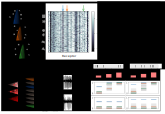
\includegraphics[width=0.95\textwidth]{figures/Figures_tuning_curve}
\caption{\textbf{A} Odor binding model. Odorants bind to olfactory receptor neurons, which may be quiescent (light gray) or active (dark gray). The likelihood that a neuron is in an active state depends on its binding affinity to constituent odor molecules (through $K^*_{i, a}$) and the energetic cost of ion channel activation. \textbf{B} Different classes of ORNs exhibit distinct binding distributions; some tuned broadly to bind many odorant molecules (blue), some specialized to a few (orange), and some weakly responding in general. \textbf{C} Example instantiation of the active binding disassociation matrix $K^*_{i, a}$ (see Methods). \textbf{D} Sample of firing activity of 9 of the 40 ORNs represented by the matrix in \textbf{C}, produced by the steady state responses (see Methods). The tuning curves, ordered for visualization, exhibit broad, specialized, and weak responses. \textbf{E} Schematic of Weber Law feedback at signal transduction. When Weber Law is enforced, firing distributions of active ORNs (shaded darkly) retain invariance with increasing signal concentrations. \textbf{F} Full activity tuning curves for the unadaptive (top) and adaptive (bottom) system, for the 3 example ORNs indicated in \textbf{B}, \textbf{C}, and \textbf{D}. Without adaptation, ORN response distribution saturates at high concentrations.}
\label{fig:tuning_curves}
\end{figure*}

Assuming that the odor binding and neuron activation process are sufficiently fast (compared to odor fluctuations), the ORN activities relax to a steady state. We first show that the steady state response reproduces observed ORN tuning curves. It is known that olfactory receptors in \textit{Drosophila} can range from narrowly tuned, responding to a single odorant, to quite broad, responding to various distinct odorants spanning multiple functional groups. We incorporate this diversity of response into our framework by treating the equilibrium disassociation constants of a odorant-receptor pair ($i$-$a$) as a random variable with pre-defined statistics. Actually, there are two disassociation constants, for the inactive and active receptor, respectively; however, for a large range of odor concentrations, the model dynamics are well dictated only by those of the active receptor, $K^*_{i, a}$, where the binding affinity is much higher. Accordingly, we only consider variations among these. 

Figure~\ref{fig:tuning_curves} shows how a simple choice of statistics on $K^*_{i, a}$ can naturally produce a diverse repertoire of response closely mimicking observed \textit{Drosophila} ORN tuning curves. The tuning curves, of which some are narrowly peaked, some are broad, and some are weakly responding, are produced by sampling at two stages. For a given receptor $a$, $K^*_{i,a}$ are chosen uniformly in some range (this dictates how receptor $a$ responds to distinct odorants), while diversity among receptors is incorporated by sampling the bounds of each range from a hyperdistribution, also chosen uniform. Receptors with narrow ranges produce peaked tuning curves (the orange ORN), while and those with broader ranges produce more disperse tuning curves (blue ORN). 


These tuning curves are maximum responses. On the other hand, it has recently been demonstrated that \textit{Drosophila} ORNs adapt their firing rates to identical background firing rates (about 30 Hz), in accordance with the Weber-Fechner law. Specifically receptor gain scales inversely with mean odor concentration, and this scaling was found to hold across various receptor and odorant identities. In our model, we incorporate this adaptive mechanism by assuming that the firing rate feeds back on the sensory machinery through the receptor free energies, $\epsilon_m$, required to produce an action potential event (see Methods). %Strictly speaking, $\epsilon_m$ are single parameter simplifications of the full dissipative process of cation inflow and membrane depolarization prior to an action potential. Nonetheless, it has been shown that adaptation in this parameter largely reproduces the Weber Scaling law 

The Weber-Fechner law is naturally incorporated into the framework of our model by scaling $\epsilon_m$ logarithmically with the mean odor concentration (between fixed outer bounds $\epsilon_{\text {L}}$ and $\epsilon_{\text {H}}$). This simple mechanism preserves firing rate response as mean odor signal increases (Fig~\ref{fig:tuning_curves}). Importantly, since this adaptive scaling acts only in response to individual OR activity levels via OR-specific free energies, the tuning curve distribution can be naturally preserved across concentration changes, irrespective of odor identity. As we will see, the maintenance of this disperse response is central to reliable odor decoding in fluctuating odor environments. 


\subsection{A combinatorial decoding process for nonlinear neural response}

\begin{figure*}
	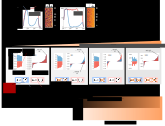
\includegraphics[width=\textwidth]{figures/Figures_signal_decoding_weber_law}
\end{figure*}


In the second stage of the discrimination framework, odorant identity is inferred from the pattern of neural response. The complicating factor in this decoding process is the disparity between measurement dimension and stimulus dimension: while \textit{Drosophila} only express 60 olfactory receptor genes, the space of aromatic odorants is $10^3$ or more, appearing to suggest that odor decoding is a fundamentally under-determined problem. However, naturally-occurring odors are comprised of only a small subset of this large space of volatile compounds. This is quite suggestive, as rigorous mathematical results show that sparse signals passed through linear sensors of sufficiently random response can be reliably reconstructed, despite measurement paucity. %This framework is known as compressed sensing. In it, an $N$-dimensional signal $\mathbf s$ is passed through $M$ sensors, producing an $M$-dimensional response vector $\mathbf y$ via the linear transformation $\mathbf y = \mathbf R \mathbf x$. This equation is not invertible since $M \le N$; compressed sensing solves this problem by instead as a convex optimization routine, simultaneously imposing both signal sparsity and the measurements as linear constraints (see Methods). 
This reconstruction technique, known in computer vision and elsewhere as compressed sensing, is naturally suited to the observed features of olfactory circuitry. %It was shown that decorrellating and diverging outputs further down the neural pathway enhance the efficacy of odor discrimination and learning. 

In compressed sensing, successful decoding relies on a sufficiently dispersed response. But large fluctuations in intensity characteristic of naturalistic environments could markedly affect response combinatorics, confounding decoding fidelity. Conversely, we expect that since imposing the Weber-Fechner scaling relation maintains the receptor activity distribution over the dynamic range of $\epsilon$, concentration-invariant accuracy can be preserved naturally over a range of odor concentrations.

To incorporate the linear framework of compressed sensing into our nonlinear receptor and activation model, we treat the odor encoding process exactly, while approximating the decoding process to first order. The latter assumption allows the compressed sensing reconstruction -- a constrained optimization problem -- to remain convex, whereby the global minimum is unique (see Methods). Specifically, we represent the nonzero components $s_k$ of the sparse odor signal $\mathbf s$ as $s_k = s_0 + \Delta s_k$, where $s_0$ is the center of the linearization. The target of the decoding process are the identities and intensities of the 'excess' signals $\Delta s_i$. The 'excess' steady state receptor activities are defined as:
\begin{align}
\Delta \bar a_m \equiv \bar a_m(\mathbf s) - \bar a_m(\mathbf s_0),
\end{align}
where we have assumed that the neural system has access to a baseline odor signal, but must infer exact odor concentrations $s_i$. The decoding process minimizes the the $L_1$ norm of $\Delta s_i$, equivalent to enforcing signal sparsity, while enforcing the linear constraints arising from the excess activities, i.e. the ORN responses (see Methods for mathematical details). To assess the decoding performance, we denote an odor signal as accurately decoded if the sparse odorant components are all estimated to within 25\% of their correct value and the components absent in the original signal, $s_j = 0$, are all estimated as less than 10\% of the mean excess concentration, $\hat s_j \le \langle \Delta s_i \rangle_i$. The former constraint is a measure of accurately inferring signal \textit{intensity}; the latter of signal \textit{identity}. 

\subsection{Identity and intensity preservation in sparse decoding with adaptive feedback}

Applying this scheme to 100 randomly chosen sparse odor signals of varying mean concentrations, we find that a large proportion are correctly inferred in a particular region of odor intensity (Fig). We find that this occurs in two different neural systems, one of which contains distinctly but all broadly responding receptors, the second of which is more indicative of \textit{Drosophila} physiology and exhibits a diverse repertoire ranging from broad to highly specialized. In both cases, however, decoding fidelity is not concentration invariant, compromising the viability of this coding scheme in naturalistic, fluctuating environments (Fig). 

Conversely, we hypothesize by stabilizing the excess activity levels through Weber-Fechner adaptive feedback, such sensitivity can be mitigated. Indeed, by enforcing a logarithmic scaling of the receptor free energies with background odor concentration, $\epsilon_m = \ln(s_0) + \epsilon_{m, 0}$, we find that the coding fidelity is now maintained over a five-fold change in odor strength. We further illustrate this behavior for systems with odorant binding distributions that are chosen exponentially and normally (Supp. Fig.). {\color{blue} What about only some receptors adapting?}



A critical feature of olfactory systems is that they can simultaneously decode odor intensity and identity, attributes which are not necessarily mutually exclusive. Compressed decoding conflates these two aspects into a single computation by inferring not only the exact component magnitudes of an odor signal (intensity), but also which molecular components constitute the high-dimensional signal in the first place (identity). Despite the conflation of these in practice, it is possible that in this framework, one aspect may be preserved while the other is violated. Separating the errors arising from each (see Methods), we find that indeed, depending on background concentration, either or both may contribute. For moderate concentrations, the inferred zero components reach a substantial fraction of the mean odor concentration, while the estimates of the sparse components are largely even with their true values (Fig.) -- the identity of the odor is substantially compromised. As concentrations increase further, identity is now preserved (zero components are estimated well below the mean), but errors in odor intensity have magnified. This illustrates that in non-adaptive systems, errors both in identity and intensity can confound odor representations, while Weber Law feedback can mitigate these conflicts. 

\subsection{Inhibitory normalization}

\subsection{Weber Law scaling permits odor discrimination amid confounding backgrounds}

\begin{figure*}
	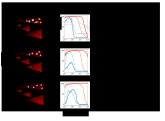
\includegraphics[width=\textwidth]{figures/Figures_signal_discrimination_weber_law}
\end{figure*}

Olfactory sensing in naturalistic settings is predicated on the ability to discriminate multiple odors, which may differ or overlap in chemical makeup and intensity. Though Weber Law adaptation can preserve single odor decoding accuracy over wide intensity range, a system which adapts to mean concentrations alone may well fail in the presence of distinct odors of largely differing concentrations. To test this, we consider two sparse odors. The first we call the "foreground" odor, and hold its odorant concentrations fixed at $s_i$. The second, which can span intensities a few orders below or above $\Delta s_0$, we refer to as the "background" odor, investigating how its intensity and identity can affect the discrimination of the foreground odorants~$s_i$. 

When the foreground odor is molecularly less complex than the background odor, the regime over which it is accurately decoded is largely identical in the adaptive and non-adaptive cases. We attribute this to the complexity of the background odor, which heavily determines the strength of adaptive feedback, irrespective of the foreground. On the other hand, the identity of the background is only correctly inferred in a particular intensity regime, which is markedly narrower in the non-adaptive case.

When the odor complexities are matched, the regime in which the foreground is correctly decoded has reduced substantially. Further, in the non-adaptive system, in only in a small range of background concentrations can both odors be simultaneously decoded accurately. This behavior magnifies as the foreground becomes more complex (Fig.). We conclude that adaptive feedback, when incorporated in a combinatorial coding scheme, aids the robust odor discrimination despite disparities in molecular complexity and intensity. 

\subsection{Dynamic adaptation preserves active odor perception in fluctuating odor environments}
We have seen that Weber Law adaptive gain can aid odor discrimination in confounding environments. So far, we have assumed that odor signals are static in time, and that adaptation from the neural circuitry feeds back onto the receptor sensitivity instantly and perfectly. But realistic odor environments are highly intermittent, and adaptation is itself dynamic. To accurately assess the role of Weber Law feedback in the combinatorial coding of naturalistic odor environments, such temporal aspects must be taken into account. 

First, we relax the assumption that adaptation is instantaneous. Instead, we assume that the firing activity of each receptor decays linearly to a given baseline level $a_{m, 0}$ through accompanying modulation of the receptor free energy. Specifically, in response to a fluctuating odor signal $s(t)$, the activity of receptor $m$ is still given by Eq. but now with time-dependent free energies, $\epsilon_m \rightarrow \epsilon_m(t)$, which obey the linear rate equation
\begin{align}
\frac{d\epsilon_m(t)}{dt} &= \frac{1}{\tau_m}\left[a_m - a_{m,0}\right],
\end{align}
where $a_m = a(s(t), \epsilon_m(t))$ is the time-dependent activity level and $\tau_m$ sets the timescale of adaptation. We compare the results for several timescales between 10 ms and several seconds.

To mimic a temporally fluctuating environment, we {\color{blue} How to explain?}. 


Considering first a set of 100 randomly chosen sparse odors, we plot the time courses of decoding accuracy, separately arising from either errors in intensity or odor identification in two windows of fluctuating odor whiffs. Specifically, we plot, over time, the percentage of correctly estimated nonzero component intensities (Fig.), as well as the the percentage of correctly identified zero components, for several distinct adaptation timescales. 

For slow adaptation, with timescales greater than a few hundred ms (lighter curves in Fig), we see definite trends in both intensity and identity coding. Errors in odor intensity are quite sensitive to the faster fluctuations in the odor signal, even if the signal remains appreciable throughout the whiff; for example the whiff demarcated by the purple and green markers in Fig.. Conversely, the majority of the odor identity is perceived as soon as the signal appears above a given whiff threshold, remaining at that level of accuracy throughout the whiff. As adaptation speed increases, the coding of odor intensity is nearly perfected within the first 100 ms of the whiff onset, remaining insensitive to further fluctuations throughout the whiff. Interestingly, odor intensity coding improves steadily as the whiff endures, though it takes several times the adaptation timescale to minimize the errors. 

Piecing this out in a bit more detail, we find that the latter of these -- the failure of odor identification rather than intensity -- is most acutely affected by the slower adaptation dynamics: the difference between zero component estimates at whiff onset and at whiff closure are nearly indistinguishable for long timescales, but can reduce by an order of magnitude for faster ones. Finally, we note that, while the number of mis-identified zero components may appear minor (20\% or so), this corresponds to several times the number of sparse components defining the odor signal itself, which is 7. Thus we expect that the increase from 80\% to $> 95$\% through the duration of the whiff indeed corresponds to a salient, dynamically improving perception of odor identity. 

Can the dynamics of increased odor perception be retained in presence of dynamic adaptation, fluctuating odors \textit{and} fluctuating backgrounds? We consider three cases, in which a background odor modulates on timescales roughly that of the foreground, somewhat slower, and substantially slower. To maximize potential confounds, we assume the foreground and background odors span odor intensities of roughly equal magnitude. In addition, anticipating our earlier results, we consider various levels of relative complexity among these two odors. {\color{blue} Explain how performanec is quantified}

When the timescale of background fluctuations is long, we find that performance improves markedly with adaptation speed (mis-identified zero components drop from 14 to 0 as timescale varies from 10 seconds to 0.5 seconds), but is already maximized at 500 ms, which exceeds the duration of most of the odor whiffs. In other words, contrary to the single odor case, odors are perfectly identified even when adaptive gain operates at timescales somewhat slower than the signal fluctuations. For slightly faster background fluctuations, but still slower than the foreground timescale, we see a marked degradation in performance with slower adaptation, although again the performance largely saturates at timescales of 500 ms or so. Further, there is now a strong dependence on foreground complexity; simpler foregrounds are easier to perceive above the background (number of mis-identified zero components $\sim 3$), while very complex foregrounds have a larger number of misidentified components $\sim 8$. This pattern continues when the background fluctuates as quickly as the foreground, though the performance  is only slightly degraded. Importantly, there is a monotonic gain in performance as adaptation speed increases, holding across fluctuation timescales and molecular complexity. Our key finding is that for odors that fluctuate on well-separated timescales, dynamic adaptive feedback obeying the Weber-Fechner Law and operating moderately quickly promotes the active perception of odor identity. 


\section{Discussion}

Drawing on recent evidence for the existence of the Weber-Fechner law in in \textit{Drosophila} olfactory receptor neurons~\cite{cafaro_WL, cao_WL,  srinivas_elife}, we propose a theoretical framework for the adaptive encoding and decoding of complex, dynamic odor environments. We argue that Weber's Law, when incorporated into a combinatorial coding strategy, is central to the accurate identification and discrimination of rapidly fluctuating, potentially conflicting odor signals. Our framework relies on two steps of odor encoding and decoding, respectively: (i) a nonlinear, stochastic model of odor-receptor binding and subsequent ORN firing, and ii) decompression of the linearized steady state ORN responses. In this framework, Weber Law adaptation is enforced naturally by scaling the free energy of ORN activation logarithmically with the ORN firing response. The encoding model is a generalization of the classical model of bacterial chemotaxis~\cite{tu_shimizu_berg}, and is mathematically equivalent to a recently proposed competitive binding model for ORN response~\cite{Cao_Tu_WL}, where it was shown that inclusion of inhibitory responses increases coding capacity of a distributed system of ORNs. Regarding decoding, recent works have pointed to the importance of a distributed response in inferring high-dimensional sparse signals~\cite{vijay_1, vijay_2, sharpee_zhang}. In this work, we place particular importance on the impact of intensity variations that typify odor signals in natural environments, finding that in both static and fluctuating odor landscapes, adaptive sensing at the receptor level play a central role in the simultaneous decoding of odor intensity and odor identity. 


\subsection{Maintaining a distributed response}

We showed that for static odor signals, a broadly sensing but non-adaptive system can accurately estimate odor identities, though only in a limited window of concentration. In living systems, adaptation maintains information transfer by ensuring that the sensory system stays in a regime of maximum sensitivity~\cite{information_theory_adaptation}. In compressed sensing, the fidelity of signal decoding relies also on the combinatorics of the sensor response~\cite{CS_tao, CS_donoho, CS_ganguli}. Indeed, it has been noted that \textit{diffusivity} in sensing -- here incorporated through the dispersity of binding constants -- underlies effective compression of high-dimensional sparse signals into a limited receptor space. Still, the nonlinearity of the steady state response, Eq., can affect the distributions of ORN activity as odor concentration increases. Thus, in the context of combinatorial coding, the central benefit conferred by the Weber Law scaling is not merely preventing ORN activities from saturating, but their distributions from distorting. 

Importantly, we find that the advantages of preserving combinatorial response carry over to more complex odor environments, where multiple odors must be discriminated. The ability to recognize weak odors over strong backgrounds is particularly relevant to olfaction in nature, where signal conflicts are pervasive. Absent Weber Law scaling, odor signals are mis-identified in the presence of strong backgrounds, producing accurate estimations only beyond a minimum intensity; this minimum itself increases with odor complexity. Further, the system is largely incapable of estimating both odors accurately -- true discrimination -- except in limited concentration windows. In principle, the adaptive system might also be susceptible to signal conflicts: mathematically, the activity distributions are invariant only in the limit that all odorants are of equal strength (Eq), so the large deviations of the weaker odorant concentrations from this mean value could lead to sensitive distortions in the distribution of ORN activities. Nonetheless, we find that odors at least as strong as the background can be identified irrespective of odor complexities. Likewise discrimination accuracy is more robust, preserved over sizable concentration windows. 


\subsection{??}
We tested our model on a particular combination of odor sparsity, odorant dimension, and receptor dimension, for various choices of system $K^*_{\text D}$ and odor identity. One aspect as yet unexplored is the relative distribution of different receptor types. Though ORNs of a given type project to a single glomerulus in the antennal lobe, multiplicities of one ORN class over another may still affect information transfer, assuming that responses are not noiseless (without noise, ORN multiplicities contain only redundant information). The optimality of a non-uniform receptor distribution in some environments was recently demonstrated for a linear combinatorial sensing system; a suggestive extension of this work is blah....





{\color{blue} Say some more about future experiments or something}


\subsection{Simultaneous coding of intensity and identity}

An important aspect of olfactory sensing is maintaining fidelity in encoding odor identity simultaneously with that of odor intensity~\cite{Laruents papers}. Here we find that in some situations these aspects may decouple with variations in odor environment; often, though errors in one coincide with errors in the other. As mentioned, compressed sensing naturally conflates identity and intensity, decoding the exact strength of odor signal components while relying fundamentally on the requirement that most of components are zero. In this sense, combinatorial coding and compressed sensing decoding confronts the identity-intensity confound quite naturally, perhaps moreso than in sensory systems in which stimuli are parameterized continuously (e.g. by frequency), such as vision and audition.

An intriguing result in our framework is the distinct manner in which errors in intensity and identity diminish during the active perception of an odor whiff. Even for relatively long adaptive timescales, identity perception increases monotonically as the odor persists, insensitive to ongoing fluctuations. Further, the proportion of mis-identified odorants continues falling on timescales much longer than $\tau_m$. {\color{blue} Implications?}


\subsection{Divisive normalization / timescales}


\subsection{The timescales of adaptation mechanisms}




\section{Methods}

\subsection{Stochastic odor-receptor binding model}

We model an odor as an $N$-dimensional vector $\mathbf s = \langle s_1,...,s_N\rangle$, where $s_i > 0$ are the concentrations of individual volatile molecules (odorants) comprising the odor. In addition, we assume that the odors are sparse in the space of odorants, so only $K$ components of $\mathbf s$ are nonzero, where $K \ll N$. The olfactory sensory system is modeled as a collection of $M$ distinct ORNs, each of which can be bound with any one of the odorant molecules, and can be either active (firing) inactive (quiescent). We only consider competitive binding, so an ORN is bound with one odorant at most. With $N$ possible odorants, receptor $a$ resides in one of $2N+2$ possible states, \{$R_a$, $R^*_a$, $R_a$-$s_i$, $R^*_a$-$s_i$\}, indicating receptors that are unbound/inactive, unbound/active, inactive/bound to odorant $i$, and active/bound to odorant $i$, respectively. We set $N = 100$, $K = 7$, and $M = 50$ throughout. 

The system dynamics are schematized in Fig.. In the mean-field limit, the binding dynamics of these $2N + 2$ states are described by the master equations:
\begin{align}
\frac{d[R_a\text{-}s_i]}{dt} &= k^+_{ia}s_i[R_a] - k^-_{ia}[R_a\text{-}s_i] \label{eq:Meq_inactive_bind_rate}\\
\frac{d[R^*_a\text{-}s_i]}{dt} &= k^{*+}_{ia}s_i[R^*_a] - k^{*-}_{ia}[R^*_a\text{-}s_i],\label{eq:Meq_active_bind_rate}
\end{align}
when receptor $R_a$ is either inactive (Eq.~\ref{eq:Meq_inactive_bind_rate}) or active (Eq.~\ref{eq:Meq_active_bind_rate}). Further, transitions between inactive and active states are described in the mean limit via:
\begin{align}
\frac{d[R_a]}{dt} &= w^{\text{u}+}_a [R_a] - w^{\text{u}-}_a [R^*_a] \label{eq:Meq_unbound_act_rate}\\
\frac{d[R^*_a\text{-}s_i]}{dt} &=  w^{\text{b}+}_{ia} [R_a\text{-}s_i] - w^{\text{b}-}_{ia}  [R^*_a\text{-}s_i],
\label{eq:Meq_bound_act_rate}
\end{align}
when receptor $R_a$ is either unbound (Eq.~\ref{eq:Meq_unbound_act_rate}) or bound (Eq.~\ref{eq:Meq_bound_act_rate}). We also define corresponding disassociation constants in terms of the binding transition rates:
\begin{align}
K_{ia} = \frac{k^-_{ia}}{k^+_{ia}} \nonumber \\
K^*_{ia} = \frac{k^{*-}_{ia}}{k^{+*}_{ia}} \label{eq:Kd_def}
\end{align}
Following (!!), we assume that in steady state, the active firing state of an ORN is energetically suppressed from the inactive state through corresponding Boltzmann factors:
\begin{align}
\frac{[R^*_a]}{[R_a]} &= \frac{w^{\text{u}+}_a}{w^{\text{u}-}_a} \equiv e^{-\epsilon^{\text u}_a} \label{eq:steady_state_act_energy_unbound} \\
\frac{[R^*_a\text{-}s_i]}{[R_a\text{-}s_i]} &= \frac{w^{\text{b}+}_{ia}}{w^{\text{b}-}_{ia}} \equiv e^{-\epsilon^{\text b}_{ia}} \quad{\text{(steady state)}}\label{eq:steady_state_act_energy_bound}.
\end{align}
However, these factors are related when detailed balance is enforced. Enforcing detailed balance upon a given 4-cycle as in Fig.~(!!) gives
\begin{align}
\frac{w^{\text{u}+}_a}{w^{\text{u}-}_a}\frac{k^{*+}_{ia}}{k^{*-}_{ia}}\frac{w^{\text{b}-}_a}{w^{\text{b}+}_a}\frac{k^{-}_{ia}}{k^{+}_{ia}} \equiv 1,
\end{align}
which in conjunction with Eqs.~\ref{eq:Kd_def}, \ref{eq:steady_state_act_energy_unbound}, and \ref{eq:steady_state_act_energy_bound} gives
\begin{align}
\epsilon_a^{\text b} = \epsilon_{ia}^{\text u} + \ln\left[\frac{K_{ia}}{K^*_{ia}}\right]
\end{align}

\subsection{Odor encoding}

\subsection{Odor decoding framework}

Odors are encoded 

\subsection{Adaptation}

\begin{align}
\Delta \hat s_i &= \underset{\Delta s_i}{\text{arg min}} \sum_i^N|\Delta s_i| \\
\text{such that  \quad} 
\Delta \bar a_m &= \sum_i R_{mi}(s_0) \Delta s_i,
\end{align}
where $R_{mi}(s_0)$ is the steady state response of receptor $a$ to odorant $i$, linearized about $s_0$ (see Methods). 

Among 100 randomly chosen sparse signals, a large percentage can be correctly inferred in given regions of mean concentration, but 







The scaling adds the disorder mentioned in previous paper

TEMPORAL: discuss how the adaptive timescale here preserves stuff .. How to incorporate primacy coding?
Primacy coding -- intensity? Not coded? Also, is it Huffman coding?

The second stage of the framework is odor discrimination, which exploits a 

%An inline figure reference will look like \tfig{single}, whereas a parenthesized figure panel
%reference will be abbreviated (\fig{single}{a}). \comment{Remove `disable' from the todonotes
%package arguments to display helpful inline comments like these. Additional commands can be defined
%for different authors.} \lipsum[4]


Equations can be referenced such as and other papers as well. References
that only appear in the supplementary materials (figure captions, etc.) or online methods section
will follow the reference numbering of the main text and appear at the end of the main reference
lis.t

Important results in the supplementary data

\bibliography{bibliography}
\end{document}
